\documentclass[border=10pt]{standalone}
\usepackage{pgf,tikz,pgfplots}
\usetikzlibrary{quotes, angles}
\usetikzlibrary{positioning}
\usetikzlibrary{arrows.meta}
\usetikzlibrary{calc, shapes, automata, fit}
\usetikzlibrary{decorations.pathreplacing}
\tikzset{%
	% Specifications for style of nodes:
	base/.style = {rectangle, rounded corners, draw=black,
		%		minimum width=4cm, minimum height=1cm,
		inner sep=15pt,
		text centered, font=\sffamily}, 
	activityStarts/.style = {base, fill=blue!30},
	startstop/.style = {base, fill=red!30},
	activityRuns/.style = {base, fill=red!30},
	process/.style = {base, minimum width=2.5cm, fill=orange!15,
		font=\ttfamily},
	context/.style = {base, inner sep=5pt, align=justify, fill=blue!30}
}

\begin{document}
	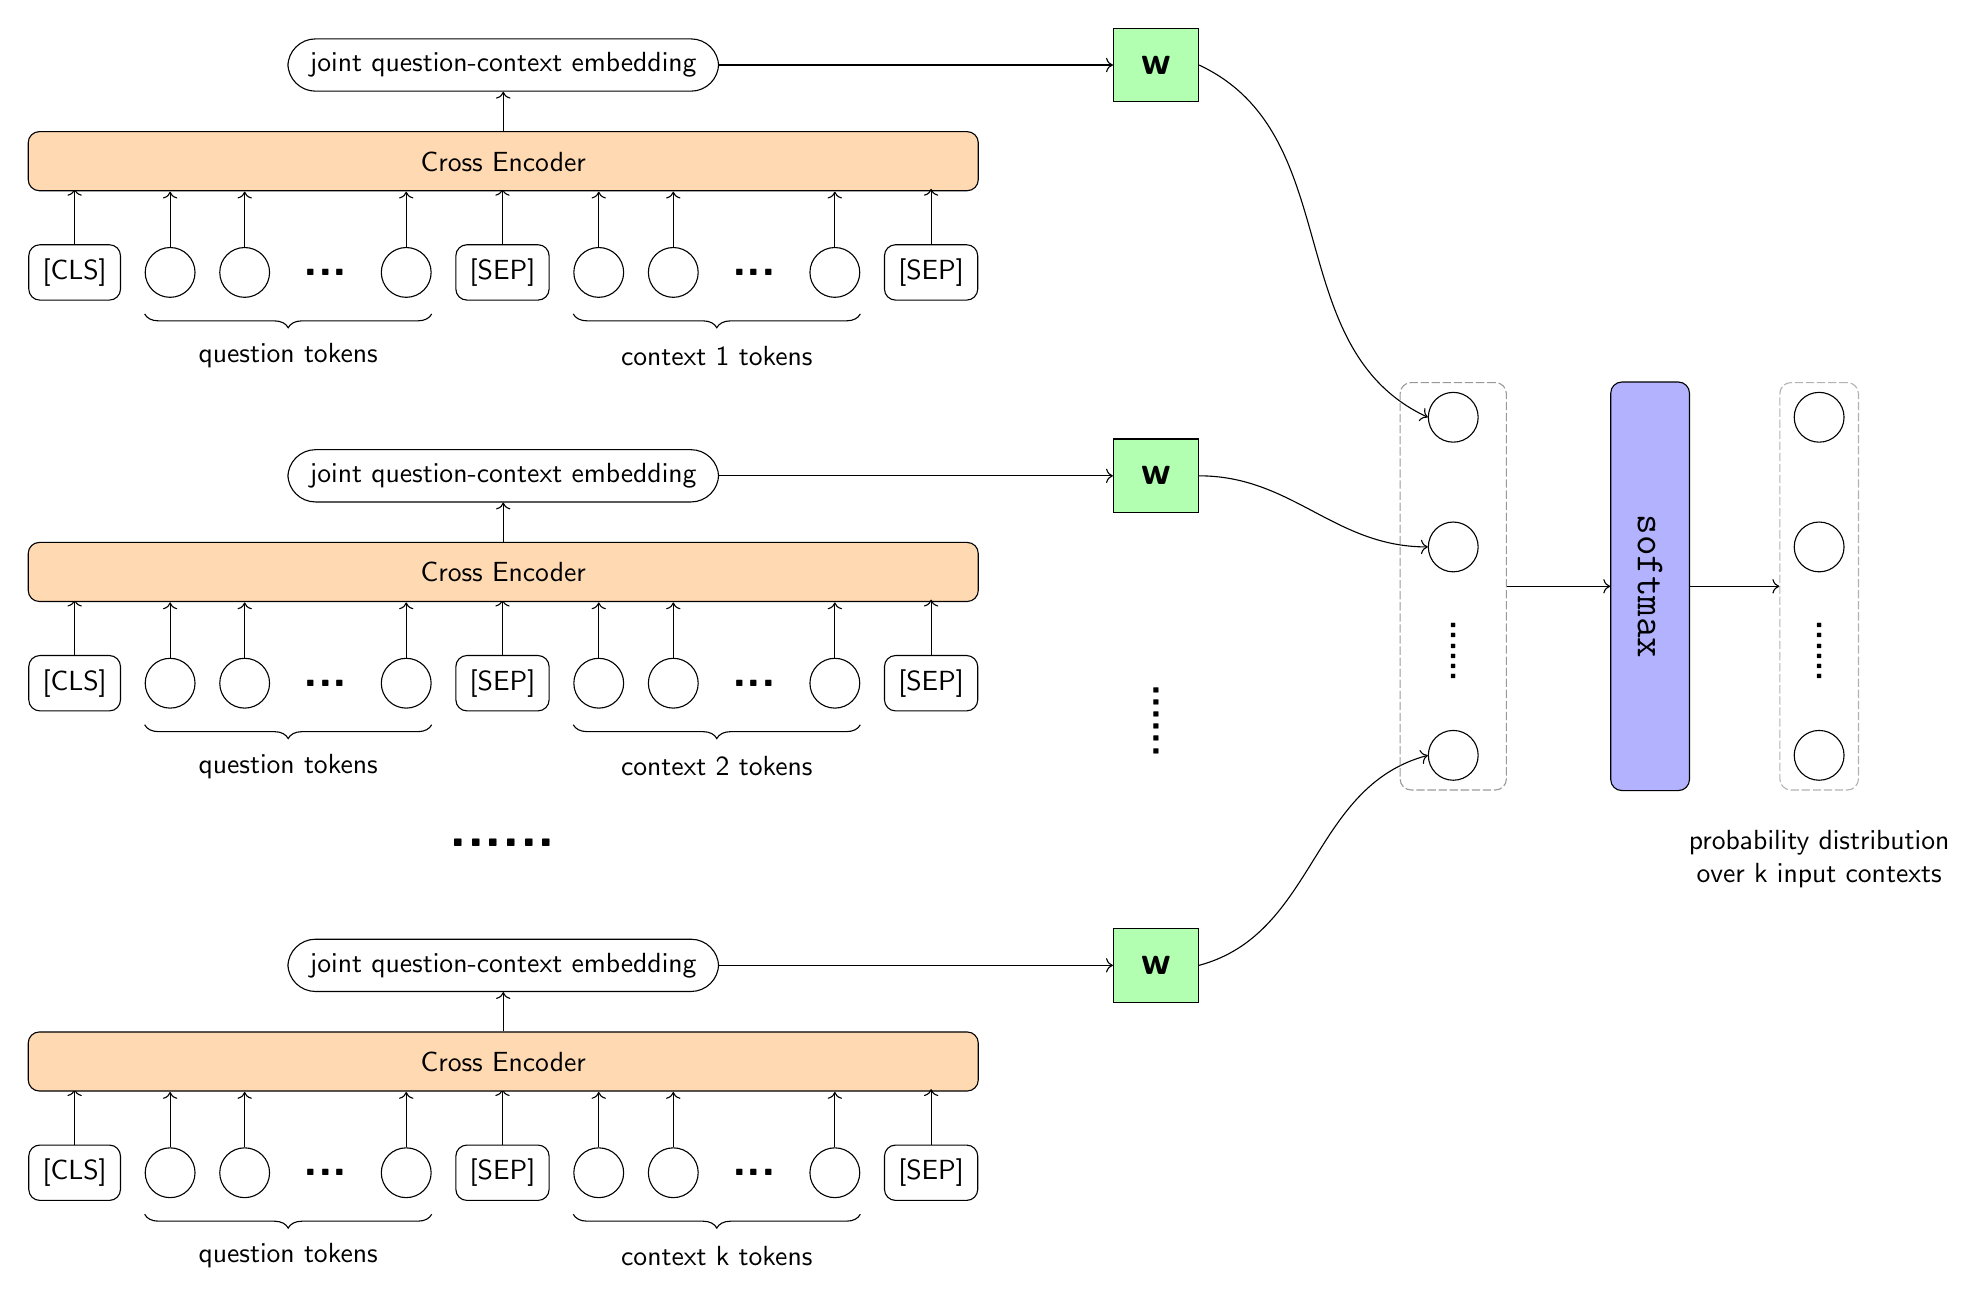
\begin{tikzpicture}[every node/.style={font=\sffamily}, align=center]
		\node [rounded corners, inner sep=5pt, draw=black] (qCLS) {[CLS]};
		\node [circle, draw=black, minimum size=18pt, right=.3cm of qCLS] (qTok1) {};
		\node [circle, draw=black, minimum size=18pt, right=.3cm of qTok1] (qTok2) {};
		\node [right=.3cm of qTok2, font=\fontsize{18pt}{\baselineskip}\selectfont\sffamily\bfseries] (qTokDots) {...};
		\node [circle, draw=black, minimum size=18pt, right=.3cm of qTokDots] (qTokLast) {};
		\node [rounded corners, draw=black, inner sep=5pt, minimum size=18pt, right=.3cm of qTokLast] (qSEP) {[SEP]};
		\draw[->] (qCLS.north) -- ++ (0., 20pt);
		\draw[->] (qTok1.north) -- ++ (0., 20pt);
		\draw[->] (qTok2.north) -- ++ (0., 20pt);
		\draw[->] (qTokLast.north) -- ++ (0., 20pt);
		\draw[->] (qSEP.north) -- ++ (0., 20pt);
		\coordinate[yshift=-15pt] (braceAnchorLeft) at (qTok1.west);
		\coordinate[yshift=-15pt] (braceAnchorRight) at (qTokLast.east); 
		\draw [decorate,decoration={brace,amplitude=5pt,mirror}] (braceAnchorLeft) -- (braceAnchorRight) node[midway, yshift=-15pt]{question tokens};
		%% Context Encoder
		\node [circle, draw=black, minimum size=18pt, right=.3cm of qSEP] (dTok1) {};
		\node [circle, draw=black, minimum size=18pt, right=.3cm of dTok1] (dTok2) {};
		\node [right=.3cm of dTok2, font=\fontsize{18pt}{\baselineskip}\selectfont\sffamily\bfseries] (dTokDots) {...};
		\node [circle, draw=black, minimum size=18pt, right=.3cm of dTokDots] (dTokLast) {};
		\node [rounded corners, draw=black, inner sep=5pt, minimum size=18pt, right=.3cm of dTokLast] (dSEP) {[SEP]};
		\coordinate[yshift=-15pt] (DbraceAnchorLeft) at (dTok1.west);
		\coordinate[yshift=-15pt] (DbraceAnchorRight) at (dTokLast.east); 
		\draw [decorate,decoration={brace,amplitude=5pt,mirror}] (DbraceAnchorLeft) -- (DbraceAnchorRight) node[midway, yshift=-15pt]{context 1 tokens};
		%% Cross encoder
		\path let
		\p1 = (qCLS.west),
		\p2 = (qCLS.north)
		in
		coordinate (qCLSAnchor) at (\x1, \y2);
		\path let
		\p1 = (dSEP.east),
		\p2 = (dSEP.north)
		in
		coordinate (dSEPAnchor) at (\x1, \y2);
		\coordinate[shift={(0., 20.pt)}] (qEncLL) at (qCLSAnchor);
		\coordinate[shift={(0., 40.pt)}] (dEncUR) at (dSEPAnchor);
		\node (enc) [fit={(qEncLL) (dEncUR)}, inner sep=0pt, draw=black, text height=0.5cm, text depth=0.25cm, fill=orange!30, rounded corners] {Cross Encoder};
		\draw[->] (dTok1.north) -- ++ (0, 20pt);
		\draw[->] (dTok2.north) -- ++ (0, 20pt);
		\draw[->] (dTokLast.north) -- ++ (0, 20pt);
		\draw[->] (dSEP.north) -- ++ (0, 20pt);
		%% output
		\node (out) [above=.5cm of enc, rounded corners=10, inner xsep=8pt, inner ysep=5pt, draw=black] {joint question-context embedding};
		\draw[->] (enc) -- (out);
		\node (mat) [right=5cm of out, draw=black, fill=green!30, inner sep=10, font=\fontsize{14pt}{\baselineskip}\selectfont\sffamily\bfseries] {w};
		\draw[->] (out) -- (mat);
		%===================================================================================
		\node [rounded corners, inner sep=5pt, draw=black, below=4.5cm of qCLS] (qCLS2) {[CLS]};
		\node [circle, draw=black, minimum size=18pt, right=.3cm of qCLS2] (q2Tok1) {};
		\node [circle, draw=black, minimum size=18pt, right=.3cm of q2Tok1] (q2Tok2) {};
		\node [right=.3cm of q2Tok2, font=\fontsize{18pt}{\baselineskip}\selectfont\sffamily\bfseries] (qTokDots2) {...};
		\node [circle, draw=black, minimum size=18pt, right=.3cm of qTokDots2] (qTokLast2) {};
		\node [rounded corners, draw=black, inner sep=5pt, minimum size=18pt, right=.3cm of qTokLast2] (qSEP2) {[SEP]};
		\draw[->] (qCLS2.north) -- ++ (0., 20pt);
		\draw[->] (q2Tok1.north) -- ++ (0., 20pt);
		\draw[->] (q2Tok2.north) -- ++ (0., 20pt);
		\draw[->] (qTokLast2.north) -- ++ (0., 20pt);
		\draw[->] (qSEP2.north) -- ++ (0., 20pt);
		\coordinate[yshift=-15pt] (braceAnchorLeft2) at (q2Tok1.west);
		\coordinate[yshift=-15pt] (braceAnchorRight2) at (qTokLast2.east); 
		\draw [decorate,decoration={brace,amplitude=5pt,mirror}] (braceAnchorLeft2) -- (braceAnchorRight2) node[midway, yshift=-15pt]{question tokens};
		%% Context Encoder
		\node [circle, draw=black, minimum size=18pt, right=.3cm of qSEP2] (d2Tok1) {};
		\node [circle, draw=black, minimum size=18pt, right=.3cm of d2Tok1] (d2Tok2) {};
		\node [right=.3cm of d2Tok2, font=\fontsize{18pt}{\baselineskip}\selectfont\sffamily\bfseries] (dTokDots2) {...};
		\node [circle, draw=black, minimum size=18pt, right=.3cm of dTokDots2] (dTokLast2) {};
		\node [rounded corners, draw=black, inner sep=5pt, minimum size=18pt, right=.3cm of dTokLast2] (dSEP2) {[SEP]};
		\coordinate[yshift=-15pt] (DbraceAnchorLeft2) at (d2Tok1.west);
		\coordinate[yshift=-15pt] (DbraceAnchorRight2) at (dTokLast2.east); 
		\draw [decorate,decoration={brace,amplitude=5pt,mirror}] (DbraceAnchorLeft2) -- (DbraceAnchorRight2) node[midway, yshift=-15pt]{context 2 tokens};
		%% Cross encoder
		\path let
		\p1 = (qCLS2.west),
		\p2 = (qCLS2.north)
		in
		coordinate (qCLSAnchor2) at (\x1, \y2);
		\path let
		\p1 = (dSEP2.east),
		\p2 = (dSEP2.north)
		in
		coordinate (dSEPAnchor2) at (\x1, \y2);
		\coordinate[shift={(0., 20.pt)}] (qEncLL2) at (qCLSAnchor2);
		\coordinate[shift={(0., 40.pt)}] (dEncUR2) at (dSEPAnchor2);
		\node (enc2) [fit={(qEncLL2) (dEncUR2)}, inner sep=0pt, draw=black, text height=0.5cm, text depth=0.25cm, fill=orange!30, rounded corners] {Cross Encoder};
		\draw[->] (d2Tok1.north) -- ++ (0, 20pt);
		\draw[->] (d2Tok2.north) -- ++ (0, 20pt);
		\draw[->] (dTokLast2.north) -- ++ (0, 20pt);
		\draw[->] (dSEP2.north) -- ++ (0, 20pt);
		%% output
		\node (out2) [above=.5cm of enc2, rounded corners=10, inner xsep=8pt, inner ysep=5pt, draw=black] {joint question-context embedding};
		\draw[->] (enc2) -- (out2);
		\node (mat2) [right=5cm of out2, draw=black, fill=green!30, inner sep=10, font=\fontsize{14pt}{\baselineskip}\selectfont\sffamily\bfseries] {w};
		\draw[->] (out2) -- (mat2);
		%================================================================================
		\node (globalDots) [below=1.5cm of qSEP2, font=\fontsize{20pt}{\baselineskip}\selectfont\sffamily\bfseries] {......};
		%================================================================================
		\node [rounded corners, inner sep=5pt, draw=black, below=5.5cm of qCLS2] (qCLS3) {[CLS]};
		\node [circle, draw=black, minimum size=18pt, right=.3cm of qCLS3] (q3Tok1) {};
		\node [circle, draw=black, minimum size=18pt, right=.3cm of q3Tok1] (q3Tok2) {};
		\node [right=.3cm of q3Tok2, font=\fontsize{18pt}{\baselineskip}\selectfont\sffamily\bfseries] (qTokDots3) {...};
		\node [circle, draw=black, minimum size=18pt, right=.3cm of qTokDots3] (qTokLast3) {};
		\node [rounded corners, draw=black, inner sep=5pt, minimum size=18pt, right=.3cm of qTokLast3] (qSEP3) {[SEP]};
		\draw[->] (qCLS3.north) -- ++ (0., 20pt);
		\draw[->] (q3Tok1.north) -- ++ (0., 20pt);
		\draw[->] (q3Tok2.north) -- ++ (0., 20pt);
		\draw[->] (qTokLast3.north) -- ++ (0., 20pt);
		\draw[->] (qSEP3.north) -- ++ (0., 20pt);
		\coordinate[yshift=-15pt] (braceAnchorLeft3) at (q3Tok1.west);
		\coordinate[yshift=-15pt] (braceAnchorRight3) at (qTokLast3.east); 
		\draw [decorate,decoration={brace,amplitude=5pt,mirror}] (braceAnchorLeft3) -- (braceAnchorRight3) node[midway, yshift=-15pt]{question tokens};
		%% Context Encoder
		\node [circle, draw=black, minimum size=18pt, right=.3cm of qSEP3] (d3Tok1) {};
		\node [circle, draw=black, minimum size=18pt, right=.3cm of d3Tok1] (d3Tok2) {};
		\node [right=.3cm of d3Tok2, font=\fontsize{18pt}{\baselineskip}\selectfont\sffamily\bfseries] (dTokDots3) {...};
		\node [circle, draw=black, minimum size=18pt, right=.3cm of dTokDots3] (dTokLast3) {};
		\node [rounded corners, draw=black, inner sep=5pt, minimum size=18pt, right=.3cm of dTokLast3] (dSEP3) {[SEP]};
		\coordinate[yshift=-15pt] (DbraceAnchorLeft3) at (d3Tok1.west);
		\coordinate[yshift=-15pt] (DbraceAnchorRight3) at (dTokLast3.east); 
		\draw [decorate,decoration={brace,amplitude=5pt,mirror}] (DbraceAnchorLeft3) -- (DbraceAnchorRight3) node[midway, yshift=-15pt]{context k tokens};
		%% Cross encoder
		\path let
		\p1 = (qCLS3.west),
		\p2 = (qCLS3.north)
		in
		coordinate (qCLSAnchor3) at (\x1, \y2);
		\path let
		\p1 = (dSEP3.east),
		\p2 = (dSEP3.north)
		in
		coordinate (dSEPAnchor3) at (\x1, \y2);
		\coordinate[shift={(0., 20.pt)}] (qEncLL3) at (qCLSAnchor3);
		\coordinate[shift={(0., 40.pt)}] (dEncUR3) at (dSEPAnchor3);
		\node (enc3) [fit={(qEncLL3) (dEncUR3)}, inner sep=0pt, draw=black, text height=0.5cm, text depth=0.25cm, fill=orange!30, rounded corners] {Cross Encoder};
		\draw[->] (d3Tok1.north) -- ++ (0, 20pt);
		\draw[->] (d3Tok2.north) -- ++ (0, 20pt);
		\draw[->] (dTokLast3.north) -- ++ (0, 20pt);
		\draw[->] (dSEP3.north) -- ++ (0, 20pt);
		%% output
		\node (out3) [above=.5cm of enc3, rounded corners=10, inner xsep=8pt, inner ysep=5pt, draw=black] {joint question-context embedding};
		\draw[->] (enc3) -- (out3);
		\node (mat3) [right=5cm of out3, draw=black, fill=green!30, inner sep=10, font=\fontsize{14pt}{\baselineskip}\selectfont\sffamily\bfseries] {w};
		\draw[->] (out3) -- (mat3);
		%===============================================================
		\path let
			\p1 = (mat2.south),
			\p2 = (mat3.north)
		in 
			coordinate (matDotsAnchor) at (\x1, \y1 / 2 + \y2 / 2);
		\node [font=\fontsize{14pt}{\baselineskip}\selectfont\sffamily\bfseries, rotate=90] (matDots) at (matDotsAnchor) {......};
		%===============================================================
		\node (neuron2) [circle, minimum size=18pt, below right=.2cm and 3cm of mat2, draw=black] {};
		\node (neuron1) [circle, minimum size=18pt, above=1.cm of neuron2, draw=black] {};
		\node (neuron3) [circle, minimum size=18pt, below=2.cm of neuron2, draw=black] {};
		\path let
			\p1 = (neuron2.south),
			\p2 = (neuron3.north)
		in 
			coordinate (neuronDotsAnchor) at (\x1, \y1 / 2 + \y2 / 2);
		\node (neuronDots) [rotate=90, font=\fontsize{12pt}{\baselineskip}\selectfont\sffamily\bfseries] at (neuronDotsAnchor) {......};
		\draw[->] (mat.east) to[out=-25, in=155] (neuron1.west);
		\draw[->] (mat2.east) to[out=0, in=180] (neuron2.west);
		\draw[->] (mat3.east) to[out=15, in=195] (neuron3.west);
		\node (logits) [fit={(neuron1) (neuron2) (neuron3)}, rounded corners, dash pattern=on 3pt off 1pt, draw=black!40, inner xsep=10pt] {};
		%===============================================================
		%softmax
		\coordinate[xshift=2cm] (softmaxUL) at (logits.north);
		\coordinate[xshift=3cm] (softmaxLR) at (logits.south);
		\node (softmax) [fit={(softmaxUL) (softmaxLR)}, inner sep=0pt, draw=black, fill=blue!30, rounded corners] {};
		\node (softmaxText) [rotate=-90, font=\fontsize{14pt}{\baselineskip}\selectfont\tt] at (softmax) {softmax};
		\draw[->] (logits) -- (softmax);
		\node (prob1) [right=4cm of neuron1, circle, minimum size=18pt, draw=black] {};
		\node (prob2) [right=4cm of neuron2, circle, minimum size=18pt, draw=black] {};
		\node (prob3) [right=4cm of neuron3, circle, minimum size=18pt, draw=black] {};
		\node (probas) [fit={(prob1) (prob2) (prob3)}, dash pattern=on 3pt off 1pt, draw=black!30, inner xsep=5pt, rounded corners] {};
		\path let
			\p1 = (prob2.south),
			\p2 = (prob3.north)
		in
			coordinate (probDotsAnchor) at (\x1, \y1/ 2 + \y2 / 2);
		\node (probDots) [rotate=90, font=\fontsize{12pt}{\baselineskip}\selectfont\sffamily\bfseries] at (probDotsAnchor) {......};
		\draw[->] (softmax) -- (probas);
		\node (probText) [below=.5cm of prob3] {probability distribution \\ over k input contexts};
	\end{tikzpicture}
\end{document}